\section{Related Work}
\label{sec:related-work}
Over the next sections I'll present the ground work for the agent I want to achieve.
Using what we've seen in \ref{sec:social-agents}, what an agent is and what it needs to have/do in order to be considered social, I'll analyse several different architectures and models that implement social agents.
%Afterwards I'll present some works related to collaborative agents since it may help in the specification of my model.
I'll then conclude with a Discussion section where I'll sum up all the pros and cons of the presented works, by this point it should be clear what I'm going to use in my model and why I'm using it.

\subsection{PsychSim}
\label{ssec:psychsim}
\begin{figure}
  \centering
    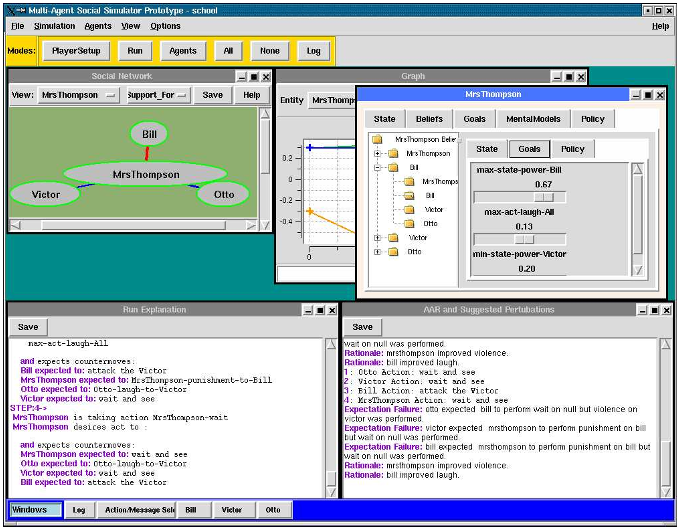
\includegraphics[width=.7\textwidth]{psychsim}
  \caption{PsychSim tool for generating new scenarios and agents.}
  \label{fig:psychsim}
\end{figure}
PsychSim \cite{marsella:psychsim} is a social simulation tool developed to explore how individuals and groups interact and how can these interactions be influenced.
The work's foundation is the fact that social interactions are based on beliefs about other's minds, a \textit{theory of mind} \cite{whiten:theoryofmind}.
Psychsim allow the users to author and explore a social scenario of his creation through the selection of generic agents models and its further specialization, see Fig. \ref{fig:psychsim}.
This tool allows users to try and understand how a specific social group might react to certain situations.

PsychSim then simulates the behaviour for each entity, individual agent or group of agents, based on their preferences, relationships, private beliefs, and mental models about each other.

In the given example, the authors explore a bullying scenario in a school and try to answer several questions:
"\textit{How might a bully respond to admonishments, appeals to kindness or punishment? 
How might other groups react in turn? 
What are the predictions or unintended side effects?}".
The simulation tool then provides explanations of the results based on each entity's preferences and beliefs, allowing the user to answer the previous questions.

PsychSim's agents are empowered with fully specified models of each other \cite{pynadath:modellingtheoryofmind}, a unique aspect of its design. Every agents maintains independent beliefs about the world, has its own goals, and it owns policies to achieve those goals. The model is composed by the state, actions, goals, beliefs, policies, messages, and mental models.

\begin{description}
\item \textbf{State} Each agent model includes a state with facts about the world, some of which may be hidden from the agent.
\item \textbf{Actions} Agents have a set of actions they can perform. Each action consists in an action type, a performer, and possibly an object of the action.
\item \textbf{Goals} These represent an agent's incentives for behaviours. In PsychSim, goals are reward functions that map the current state to a real value.
\item \textbf{Beliefs} The simulations agent have only a \textit{subjective} view of the world, where they form beliefs about what \textit{they} think is the state of the world. An agent's beliefs consists in models of all agents (including himself), representing their state, beliefs, goals, and policy of behaviour.
\item \textbf{Policies} Each agent's policy is a function that represents the process by which it selects an action or message based on its beliefs and goals.
\item \textbf{Messages} Messages are attempts by one agent to influence the beliefs of recipients and have five components: a source, recipients, a message subject, content, and overhearers.
\item \textbf{Mental Models} An agent's beliefs about another agent are realized as a fully specified agent model of the other agent, including goals, beliefs, and policies. Mental Models are predefined models which represent agents goals, beliefs, and policies.
\end{description}

As a social agent architecture, PsychSim presents a well-defined model capable of fully simulating social behaviour.
It is based on sound theories from psychology (theory of mind) and has into account other agents in its cognitive process, a requirement for social agents as we saw in \ref{ssec:social-agents}.

However, PsychSim lacks planning capabilities.
Based only of policies to guide it's immediate behaviour, each agent will follow the scenario devised by the user disregarding any future states.
\subsection{Comme il Faut}
\ac{CiF} is an \ac{AI} system that enables authors to create interactive stories by specifying, not the complete narrative and all its ramifications but, high-level rules governing expected character behaviour given social situations \cite{mccoy:cif-social-story-worlds}.
In \ac{CiF}, characters use many attributes of the current social state, including the story of prior interactions, to decide how to engage in social exchanges with other characters.
This architecture provides a rich social environment for characters to interact allowing the creation of dynamic and interactive stories.

\ac{CiF} does not store world information in a series of events, like many \ac{AI} techniques do (e.g. Behaviour Trees and Hierarchical Task Networks).
Social exchanges are the primary structure of representing knowledge in \ac{CiF} \cite{mccoy:cif-authoring}.
They consist in social interactions between characters that modify the social state of the participants.
By using social exchanges and additional encoded social context, \ac{CiF} lowers the authoring burden needed to create the social aspects of an interactive story by allowing the author to specify the rules and general patterns of how social interaction should take place.

Characters' behaviour is chosen based on rules in a large rule database that depict normal social behaviour in a particular story world.
These rules in conjunction with the logic of a social world, a set of characters, and a series of scenario goals allows \ac{CiF} to determine the desired action for each character.

\ac{CiF} provides a sound model for empowering characters with social ability, but it's main goal is storytelling.
As an architecture for an agent, it lacks planning capabilities that we need for our agent.
Despite its successful implementation in the game Prom Week \cite{mccoy:prom-week} \footnote{Mismanor, a still in development role-playing game that uses an altered version of \ac{CiF}, is another example.}, the authors still need to specify every rule for every possible social interaction between characters. Prom Week contains over forty nine hundred unique influence rules, around sixty social exchanges with over twenty rules that contribute to the characters desire and responses, a cast of eighteen characters, and a combined total of over forty thousand predicates.
\subsection{Fatima}
\subsection{Versu}
Versu is a text-based interactive drama available in the App Store for the iPad\footnote{You can visit the game webpage at https://versu.com.}, see Fig. \ref{fig:versu}  \cite{evans:versu}.
One of the game's appeal is its high re-playability due to the use of autonomous agents (the user can play the same episode several times with different results).

\begin{figure}
  \centering
    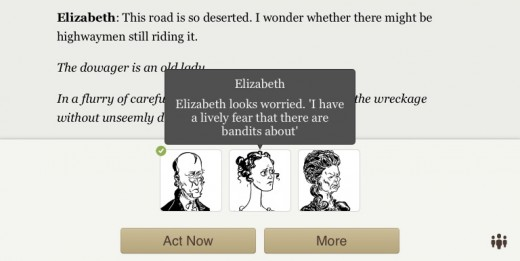
\includegraphics[width=.7\textwidth]{versu}
  \caption{An example of Versu's game play.}
  \label{fig:versu}
\end{figure}

The game is based upon two objects: agents and social practices.
Social practices describe a recurring social situation that may exist only for a short time (e.g. a conversation, a game, a meal) or can last much longer (e.g. a family, the moral community).
These practices coordinate agents via the \textit{roles} they are playing and their main function is to describe the actions the agents can do in each situation.

Social practices provide the agent with a set of suggested actions, but it is up to the agent himself to decide which action to perform, using utility-based reactive action selection (the utility is calculated in accordance with the agents beliefs, desires, personality quirks, and backstory).

Versu's world allows multiple practices to exist concurrently. For example, in a dinner party, there will be multiple practices operating at once:
\begin{itemize}
\item eating and drinking.
\item the conversation about politics
\item the rising flirtation between Frank and Lucy
\item responding to the fact that Mr. Quinn has spilled the soup.
\end{itemize}

Performing an action can result in any sentence being added to the world database.
The results of adding new sentences can be that relationships are updated, new beliefs or desires are formed, old practices are deleted or new practices are spawned.

Agents and social practices are scripts authored in a high-level \ac{DSL} designed specifically for this simulation: Praxis\footnote{Praxis is based on Exclusion Logic \cite{evans:exclusion-logic}, a new deontic logic.}.

Versu's success is proof that the architecture can produce social agents with high adaptability.
But, as some of the already explored works, Versu's agents lack planning capabilities.
It's logic powered approach is a differentiating aspect from the previous models, however it does imposes some limitations.
One example is how the agents beliefs are expressed.
The system cannot represent universal and existential quantifiers (e.g. "everyone has become insane" and "the murderer is one of the guests", respectively) or beliefs about others' beliefs (e.g. "Mr Quinn believes that Lucy believes that Mrs Quinn is the murderer").

\subsection{dorgoly-social-agents}

%\subsection{Working Together}
In \ac{DST}, a multi-player game, players will often come across each other and may work together in order to achieve a goal (e.g. defeating a giant).
Working together may become a substantial part of the agents activities.
Thus, it is important to understand how agents can work together.

\subsubsection{Joint Intentions}
What is involved when a group of people decide to do something together?
Joint action by a team involves more than just the union of simultaneous individual actions, even when those actions are coordinated. We would not say that there is any team work involved in ordinary automobile traffic, even though the drivers act simultaneously and are coordinated by the traffic signs and rules of the road.

But when a group of drivers decide to do something together, such as driving somewhere as a convoy, it appears that the group acts as a single agent with beliefs, goals, and intentions of its own, over and above the individual ones.
Levesque proposed a formal model of these mental properties of a group, and especially how joint intentions to act affect and are affected by (and ultimately reduce to) the mental states of the participants \cite{levesque:joint-intention}.

In his work, Levesque argues that groups of agents have joint intentions.

\subsubsection{SharedPlan}

\subsubsection{STEAM}
STEAM is an implemented general model of teamwork based on \textit{joint intentions} theory \cite{levesque:joint-intention} and the \textit{SharedPlans}\footnote{This theory is based on a intentional attitude, \textit{intending that}, which represents an agent's intention towards its collaborator's actions.} theory \cite{grosz:sharedplan}.

STEAM starts with joint intentions but then builds up hierarchical structures that parallel the SharedPlans theory, particularly, partial SharedPlans.
The result is a hybrid model of teamwork, that borrows from the strengths of both joint intentions (formalization of commitments in building and maintaining joint intentions) and SharedPlans (detailed treatment of team's attitudes in complex tasks, as well as unreconciled tasks).

\subsection{Discussion}
Throughout the previous sections we've looked at social agents and some works that use and implement social agents.
%We've also taken a look at collaborative agents with the purpose of defining a model to implement a social agent.
There are several aspects that an agent must possess in order to be considered social, as discussed in \ref{sec:social-agents}.
Keeping in mind that the agent's actions must be social by design, the key capability of a social agent is mind-reading.

All of the explored architectures have mind-reading capabilities provided by the use of \ac{TOM} models.
\ac{TOM} models allow the agent to include other agents perceived intentions and desires in its deliberative process (either in choosing a single action or in its planning processes).
Versu's \ac{TOM} model is based on exclusion logic.
Although powerful, this representation encompasses limitations on what we can express as we saw in \ref{sec:versu}.
On another hand, PsychSim's agents are empowered with fully specified models of each other.
However, these mental models are predefined, an ill-suited option for the agent since it will be dealing with unknown human players.
Dorgoly's architecture, however, presents a much more versatile approach in which every event will continuously construct the models of other agents.

One of the main points argued was the planning capabilities of the architectures/models.
Planning is paramount for the agent as it may imply the agent's survival \footnote{As we've previously seen in \ref{sec:dst} the agent must be able to prepare himself, for example, to last through Winter scarcity of resources. }.
As we've seen, PsychSim, \ac{CiF}, and Versu lack this ability while \ac{FAtiMA} and Dorgoly's architecture don't.
However, Dorgoly's architecture use of roles (social context) in influencing planning, provides a straightforward medium make the agent's actions social.

Although it was not a requirement, both \ac{FAtiMA} and Dorgoly's architecture made use of appraisal theories to model emotions.
This is also significant for this work's purpose.
Expressing emotions is one key aspect of believability \cite{bates:believable-agents}, which can help players in engaging with the agent.
The use of a believable agent will help in improving the game play experience of the players, our main objective.

Finally, Dorgoly's architecture distinguishes itself by its use of roles to model social context.
Through the use of roles we can influence the character's reactions and behaviour (e.g. when in the presence of a friendly player, the agent may pro-actively ask for help), making the agent social by nature.

To summarize, these works have all contributed to the design of the proposed solution in the next section.
Their use of \ac{TOM} models, memory, and emotions will all be encompassed in the solution.
However, one work stands out has the most influencing one, Dorgoly's dissertation: An Architecture for Believable Socially Aware Agents.
The proposed solution is heavily based upon Dorgoly's  work, being in fact, an adaptation of it.